\let\oldthesubsection=\thesubsection
\renewcommand{\thesubsection}{\Roman{subsection}}

A dolgozat olyan nyelvtechnológiai előfeldolgozó algoritmusokat mutat be, melyek hatékonyan képesek szövegek elemzésére agglutináló nyelvek esetén. 
Vizsgálataimat magyar nyelvre végeztem, de a módszerek kidolgozása során törekedtem a nyelvfüggetlenségre. 
Így, a bemutatott eljárások más, hasonló struktúrájú nyelvek esetén is sikerrel alkalmazhatóak.
%Munkám során kiemelt szerep jutott a morfológiai egyértelműsítés feladatának, mivel ennek kimenetére számtalan információkinyerő rendszer épít.

Az első téziscsoportban a általános magyar nyelvű morfológiai egyértelműsítés területén elért eredményeimről számolok be. 
Ezt követően bemutatom a létrehozott annotáló eszköz egy gyakorlati alkalmazását. 
Végül, ismertetem azon új előfeldolgozó eljárásokat, melyek zajos (klinikai) szövegeket is hatékonyan képesek elemezni.

\subsection{Hatékony morfológiai egyértelműsítő algoritmusok}
\label{thes:morf}

A morfológiai egyértelműsítés egy olyan összetett probléma, mely a szófaji címkék meghatározásából és a szavak lemmatizálásból áll. 
Míg az első részfeladatot a szakirodalom megoldottnak tekinti, addig az utóbbi területen sokkal kevesebb fejleményről számolhatunk be. 
A téziscsoport először egy szótövező módszert ismertet, majd leírja a teljes morfológiai egyértelműsítés során alkalmazott módszeralgoritmusokat.

\begin{core}
\begin{thesis}\label{thes:morf-lemma}
Kidolgoztam egy olyan algoritmust, ami agglutináló nyelvek, így magyar esetén nagy pontossággal képes szavak lemmáit azonosítani. 
Az eljárás a tanítóanyagban látott szavakon túl az ún. ismeretlen szóalakokat is képes hatékonyan kezelni, amihez a morfológiai elemző lehetséges elemzésein kívül a tanítóanyagból épített statisztikai modellekre is épít. 
Mérésekkel kimutattam, a módszer magyar nyelv esetén kimagasló pontossággal bír. 
\end{thesis} 

\begin{pub}
\cite{Orosz2011,Orosz2012,Orosz2012a,Orosz2013a}
\end{pub}
\end{core}

Az algoritmus két fázisban végzi a szótövesítést. 
Első lépésben meghatározza a szó lehetséges lemmáinak halmazát. Ehhez felhasználja a morfológiai elemző javaslatait illetve egy ismeretlenszó-elemző kimenetét is. 
Ezt követően a jelöltek ($l$) mindegyikéhez a szóalak ($w$) és az előzetesen kalkulált morfoszintaktikai címke ($t$) függvényében valószínűségi értékeket számol:
\begin{equation}\label{lemma-interpolated}
P(l|w,t) = P(l)^{\lambda_1} P(l,t|w)^{\lambda_2}
\end{equation}
Az így kapott interpolált algoritmus egy egyszerű gyakorisági eloszlást és egy szóvég-alapú valószínűségi modellt kombinálva határozza meg a legmegfelelőbb lemmát.

Megmutattam, hogy az új szótövező algoritmus kiemelkedő pontossággal bír magyar nyelv esetén. %TODO: ehhez vannak-e számok, alátámasztható-e
%Összevetve a baseline (MLE becslésen alapú) metódussal annak hibáit mintegy XX\%-kal képes csökkenteni XX\%-os pontosságot eredményezve.


\thesisline%%%%%%%%%%%%%%%%%%%%%%%%%%%%%%%%%%%%%%%%%%%%%%%%%%%%%%%%%%%%%%%%%%%%%


\begin{core}
\begin{thesis}\label{thes:morf-tagging}
Létrehoztam egy olyan hibrid morfológiai egyértelműsítő eszközt (PurePos), mely hatékonyan alkalmazható  morfológiailag komplex és nyelvi erőforrásokban szegény nyelvek esetén. 
Az algoritmus statisztikai eljárásokra támaszkodva, morfológiai elemző integrált alkalmazásával és szabály alapú komponensek használatával hatékony egyértelműsítést tesz lehetővé. 
Megmutattam, hogy az eljárás magyar nyelv esetén state-of-the-art pontossággal rendelkezik (akár nagyon kevés tanítóanyag esetén is).
\end{thesis}

\begin{pub}
\cite{Orosz2011,Orosz2012,Orosz2012a,Orosz2013a}
\end{pub}
\end{core}

\begin{figure}[ht] 
  \centering
  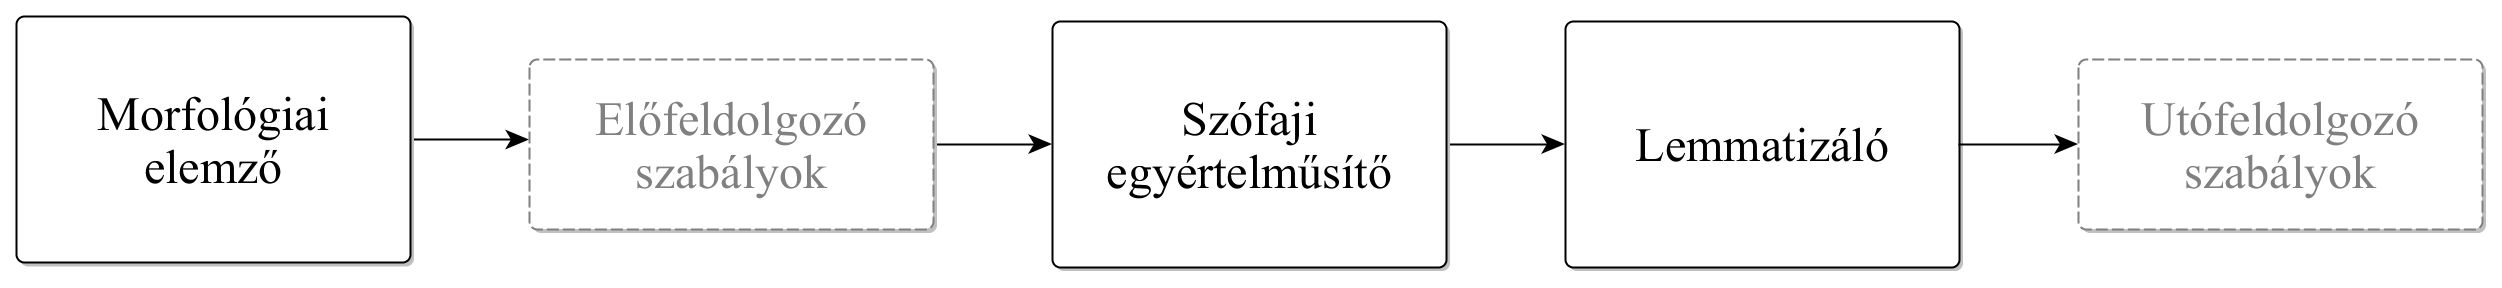
\includegraphics[width=1\textwidth]{MorphTagging/architecture_hu.png} 
  \caption{A hibrid morfológiai egyértelműsítő algoritmus architektúrája}
  \label{fig:purepos-arch_hu}
\end{figure}

A rendszer architektúráját  (ld. \ref{fig:purepos-arch_hu} ábra) úgy alakítottam ki, hogy a statisztikai modulokon túl szimbolikus komponensekkel is hatékonyan tudjon együttműködni. 
Ily módon a címkék és szótövek azonosítása több lépésben történik:
az egyértelműsítés alapját egy morfológiai elemző képezi, melyet több lépésben sztochasztikus algoritmusok követnek. 
%Ezen eljárások elemző kimenetére épülve hozzák meg döntéseiket. 
A szófaji egyértelműsítés folyamata olyan létező algoritmusokra épül, melyeket korábban más sikeresen használtak agglutináló nyelvek elemzésére. 
A felhasznált trigram-alapú metódust úgy adaptáltam, hogy azok hatékonyan működjenek morfológiailag komplex nyelvek esetén is.
A szófaji címkézést követően, az elemzés utolsó fázisában történik a lemmák meghatározása a \ref{thes:morf-lemma} tézisben bemutatott módon.

\begin{figure}[H]
  \centering
  \includegraphics[width=1\textwidth]{MorphTagging/msd_token_hu.png}
  \caption{Morfológiai egyértelműsítő algoritmusok tanulási görbéje}
  \label{fig:humor-token_hu}
\end{figure}


Méréseimmel megmutattam, hogy a teljes egyértelműsítő algoritmus kimagasló pontossággal bír magyar nyelv esetén. 
Ehhez a PurePos rendszert a Szeged Korpusz 2.3-as változatán 80\%-n tanítottam és a maradékon mértem a hatékonyságát. 
A rendszer így 96.27\%-os szószintű pontosságot nyújt.
Vizsgáltam még az eszköz alkalmazhatóságát olyan esetekben, mikor csak kevés tanítóanyag áll rendelkezésre.
Kimutattam, hogy a PurePos ilyenkor is nagy pontossággal alkalmazható (vö. \ref{fig:humor-token_hu} ábra). 
Ismertettem még az eljárás egy olyan alkalmazását, ahol a hibrid komponenseinek köszönhetően mintegy 68\%-kal sikerült javítani az eredeti elemzőlánc pontosságán, így jelentősen gyorsítva a manuális annotációs folyamatot.


\thesisline%%%%%%%%%%%%%%%%%%%%%%%%%%%%%%%%%%%%%%%%%%%%%%%%%%%%%%%%%%%%%%%%%%%%%


Bár a \ref{thes:morf-tagging} tézisben ismertetett algoritmusok magas pontossággal rendelkeznek, megmutattam, hogy ezek teljesítménye tovább növelhető más rendszerekkel való kombinációval. 

\begin{core}
\begin{thesis}
Létrehoztam egy olyan módszert, mely morfológiai egyértelműsítő rendszerek kombinációjával kimagasló pontosságot ér el magyar nyelv esetén.
A kidolgozott eljárás újdonsága, hogy külön alrendszerekben végzi a lemmák és morfoszintaktikai címkék azonosítását, majd azok kimenetét egyesítve végzi az egyértelműsítést.
Ezen felül példány alapú tanulásra épül, s úgy kapcsolja össze az egyes rendszerek eredményeit, hogy azok és a kombináló algoritmus is a teljes tanítóanyagból tudnak tanulni. 
Méréseimmel alátámasztottam, hogy az egyesítő módszer teljesítménye jelentősen meghaladja a felhasznált eszközök pontosságát. 
\end{thesis}

\begin{pub}
\cite{Laki2013a,Orosz2013c,Orosz2013d} 
\end{pub}
\end{core}

Első lépésként, kidolgoztam egy új metrikát (OER), ami effektíven képes egyértelműsítő rendszerek hibáinak különbözőségét vizsgálni. 
Ezt felhasználva megmutattam, hogy a HuLaPos rendszer tipikus hibái eltérnek a PurePos-étól. 
Az általános kombinációs algoritmusok eredményességének részletes vizsgálata után, olyan jellemzőhalmazokat hoztam létre, melyek morfológiailag komplex nyelvek esetében magasabb pontossággal használhatóak.
Ezt követően kidolgoztam egy olyan eljárást melyben két külön komponens választja ki a szófaji címkéket illetve a lemmákat. 
A kombinációs rendszer moduljai keresztvalidáció segítségével tanítják az első szintű osztályozókat, amik példány alapú tanulásra épülnek.

Megmutattam, hogy az új algoritmus a PurePos hibáinak mintegy 28,90\%-át javítja. 
Eredményeimmel igazoltam, hogy egy teljes egyértelműsítő algoritmus pontossága jelentős mértékben javítható egy másik rendszerrel való kombinációval. 

\subsection{Morfoszintaktikai komplexitás automatikus becslése morfológiai egyértelműsítő algoritmusok alkalmazásával}
\label{thes:mlu}

A morfológiai komplexitás mérése fontos eszköze a nyelvfejlődést mérő kutatásoknak.
Ezt agglutináló nyelvek esetén a megnyilatkozások átlagos morfémában mért hosszával (MLUm) számolják.
Míg angolra és más morfológiailag nem összetett nyelvre léteznek automatikus eljárások MLUm számolásra, 
addig magyarra (és hasonló agglutináló nyelvekre) ezek nem alkalmazhatóak. 
Így tehát ezekben az esetekben a megnyilatkozások hosszának mérése csak időigényes manuális számolással lehetséges.

Dolgozatomban megmutattam\footnote{A morfológiai komplexitás becslésének feladatát Mátyus Kingával együtt végeztem. A korpusz manuális címkézése, az annotálás útmutató kidolgozása közös munka eredménye. Az MLUm becslés nyelvészeti alapvetései a társzerző érdeme, míg a folyamat algoritmizálása önálló eredmény.}
, hogy a PurePos rendszer egy megfelelő morfológiai egyértelműsítővel kiegészülve adekvát alapja egy automatikus morfémaszám-becslő eljárásnak, és így kiváltja a fáradtságos emberi munkát. 

\begin{core}
\begin{thesis}
\label{thes:spoken-morf-tagging}
Létrehoztam egy  hibrid morfológiai egyértelműsítő láncot beszédátiratok nagy pontosságú elemzésére. 
Az algoritmus alapját az \ref{thes:morf-tagging} tézisben ismertetett rendszer képezi, melyet a beszélt nyelv címkézéséhez szükséges szabályokkal adaptáltam. 
Méréseimmel igazoltam, hogy a létrejött elemzési lánc teljesítménye megközelíti az általános nyelvi egyértelműsítők eredményességét.
\end{thesis}

\begin{pub}
\cite{Matyus2014,Orosz2014c}
\end{pub}
\end{core}

Az teljes egyértelműsítő rendszer a Humor morfológiai elemzőre épül, melyet a beszélt nyelvben tipikus jelenségekkel egészítettem ki. 
A morfológiai elemző kimenetére épülve a PurePos végzi a lemmák és címkék meghatározását, melyet szabály alapú eljárásokkal adaptáltam a doménhez.

Az egyértelműsítő lánc pontosságának méréséhez létrehoztunk egy 1000 megnyilatkozásból álló etalon korpuszt, melyek a MONYEK \cite{Matyus2014} korpusz részét képezik. 
Az annotáció folyamatához kidolgoztuk egy az eddigiektől eltérő, beszélt nyelvre adaptált címkekészletet, majd létrehoztunk egy annotálási útmutatót.

Vizsgálataimmal alátámasztottam, hogy a PurePos rendszer nagy pontossággal használható magyar nyelvű beszédátiratok elemzésére. 
A bemutatott szabály alapú és statisztikai technikák alkalmazásával 96\%-os szószintű pontosságot értem el, mely megközelíti az általános nyelvi egyértelműsítőkét.


\thesisline%%%%%%%%%%%%%%%%%%%%%%%%%%%%%%%%%%%%%%%%%%%%%%%%%%%%%%%%%%%%%%%%%%%%%


\begin{core}
\begin{thesis}
\label{thes:mlu-estimation}
Kifejlesztettem egy olyan új eljárást, ami beszédátiratok morfoszintaktikai összetettségét képes automatikusan becsülni.
Az algoritmus a \ref{thes:spoken-morf-tagging} tézisben bemutatott elemzőláncra épülve, annak kimenetében számolja a megnyilatkozások morfémában mért hosszát. 
Méréseimmel kimutattam, hogy a módszer eredménye nagy mértékben korrelál az humán elemzők által számolt MLUm értékekkel.
\end{thesis}

\begin{pub}
\cite{Matyus2014,Orosz2014c}
\end{pub}
\end{core}

Az algoritmus a szavak morfoszintaktikai annotációjára épülve összegzi a megnyilatkozások morfémáit.
A bemutatott éljárás a Humor elemző számára ismeretlen szóalakok hosszára is képes becslést adni.
Ezeken túl az MLUm értékekhez nyelvészetileg releváns szabályokat valósít meg.

Az módszer tökéletesítéséhez létrehoztunk egy morfémaszámokat is tartalmazó etalon korpuszt. 
Megmutattam, hogy az automatikus módszer 0,9901 korrelációs értékkel bír, míg az átlagos relatív eltérése csupán 4,49\%. 
Méréseimmel bebizonyítottam, hogy az eljárás alkalmas az időigényes manuális morfémaszámolás kiváltására.

\subsection{Zajos szövegek hatékony elemzése}
\label{thes:clin}

Napjainkban egyre több elektronikusan rögzített dokumentum keletkezik klinikai környezetben, melyek nagy mennyiségű eddig el nem érhető közvetett tudást reprezentálnak. 
Mivel létrehozásuk során nem fordítanak figyelmet a szövegek struktúrájának kialakítására és a helyesírási normák betartására, így azok feldolgozása gyakran nem megoldható létező eszközök közvetlen alkalmazásával. 
Bár angol nyelvre számtalan megoldás született az évek során, a magyar (és más morfológiailag összetett) nyelvű orvosbiológiai szövegek elemzése egy eddig nem vizsgált terület.

% \begin{core}
% \begin{thesis}
% 
% \end{thesis}
% 
% \begin{pub}
% \cite{Orosz2013d, Orosz2014a}
% \end{pub}
% \end{core}


%%%%%%%%%%%%%%%%%%%%%%%
% \thesisline%%%%%%%%%%%%
%%%%%%%%%%%%%%%%%%%%%%%

\begin{core}
\begin{thesis}%{II.1/b}
\label{thes:clin-segment}
Létrehoztam egy olyan hibrid eljárást, mely magyar nyelvű klinikai rekordokat képes magas pontossággal mondatokra és szavakra bontani. 
A módszer alapját egy hagyományos szabály-alapú szegmentáló eszköz képezi, amit olyan felügyelet nélküli gépi tanulást használó módszereket készítettem, melyek hatékonyan képesek javítani a teljesítményén.
Méréseimmel alátámasztottam, hogy a hibrid rendszer által azonosított mondat- és szóhatárok kellően pontosak a gyakorlati alkalmazhatósághoz.
Ezeken túl kimutattam még, hogy a magyar nyelvre elérhető algoritmusok közül sem a szabályalapú, sem a gépi tanulást használó rendszerek nem alkalmasak orvosbiológiai szövegek tokenizálására és mondatrabontására.
\end{thesis}

\begin{pub}
\cite{Orosz2013d, Orosz2014a}
\end{pub}
\end{core}

A bemutatott szegmentáló algoritmus alapját szabály-alapú, mintaillesztést használó algoritmusok képezik. 
Ezek bár magas pontossággal bírnak fedésük alacsony, így ezt felügyelet nélküli, gépi tanuló eljárásokkal bővítettem.
Megmutattam, hogy a módosított $\log \lambda$ módszer nagy mértékben lehetséges növelni a rendszer fedését. 
A teljesítmény javításához a szóalakok felszíni jegyein túl, a Humor elemzéseit is beépítettem.


A mérésekhez létrehoztam egy manuálisan javított korpuszt, amin az egyes rendszerek szószintű és mondatszintű pontosságát, fedését és a kombinált $F$-értét is vizsgáltam.  
Kutatásomban a speciálisan magyar nyelvre fejlesztett rendszereket, illetve egy maximum entrópia módszeren alapuló gépi tanulásos algoritmust is kiértékeltem.

Mérésekkel alátámasztottam, hogy a mondatrabontás feladatában a legtöbb elérhető rendszer 50\%-os $F$-érték alatt teljesít. 
Ezek alól csak két eszköz képezett kivételt, de egy részletes elemzésben rávilágítottam, hogy azok kimenete sem alkalmas további feldolgozó rendszerek bemenetéül.
Ezekkel szemben méréseimmel megmutattam, hogy az új hibrid algoritmus mind a mondatokra mind pedig a szavakra bontás tekintetében 90\% feletti $F$ értéket produkál. 
Következésképpen az ismertetett algoritmusok alkalmasak magyar nyelvű klinikai dokumentumokban szó- és mondathatárok azonosítására.

%%%%%%%%%%%%%%%%%%%%%%%
\thesisline%%%%%%%%%%%%
%%%%%%%%%%%%%%%%%%%%%%%

\begin{core}
\begin{thesis}%{II.2}
\label{thes:clin-pos}
Megmutattam, hogy az \ref{thes:morf-tagging} tézisben ismertetett rendszer, megfelelő szimbolikus algoritmusokkal kombinálva alkalmas orvosbiológiai szövegek elfogadható minőségű automatikus morfológiai egyértelműsítésére. 
Méréseimmel kimutattam, hogy a szabály alapú és statisztikai doménadaptációs technikák jelentős mértékben javítanak az elemzési lánc pontosságán.
\end{thesis}

\begin{pub}
\cite{Orosz2013,Orosz2014b} 
\end{pub}
\end{core}

Az eljárás a Humor morfológiai elemző egy bővített változatára és a PurePos egyértelműsítő rendszerre épül. 
Dolgozatomban feltártam egy általános nyelvi elemzőlánc tipikus hibáit és a rendszer számos hiányosságát orvosoltam doménspecifikus szabályok alkalmazásával. 

A mérések elvégzéséhez létrehoztam egy ki méretű etalon korpuszt, melynek morfológiai annotációját manuálisan javítottam. 
Megmutattam, hogy a közreadott rendszer szószintű pontossága (93.73\%) jelentősen meghaladja a baseline lánc teljesítményét (88,09\%). 

A bemutatott szegmentáló és egyértelműsítő eljárások hibái a rövidítések kezelésének nehézségeiből fakadtak, így a jövőben indokolt lehet egy olyan módszer kidolgozása, mely a két feladatot egyszerre célozza meg.

\let\thesubsection=\oldthesubsection
